\subsection{Model Setup \& Methodology}\label{sec:dem-setup}
We analyze a three-dimensional pebble bed consisting of mono-dispersed particles of diameter $d_p$. The particles are constrained by rigid $y-z$-planes at locations of $\frac{x}{d_p} = \pm 10$ (the walls of our container). There are periodic boundary conditions in the $y$-direction located at $\frac{y}{d_p} = \pm 7.5$. Gravity acts in the negative $z$-direction and the particles are resting on a rigid $x-y$-plane at $z=0$ (the floor of the container) and held from the top by an $x-y$-plane at $\frac{z}{d_p} = 30$ (the roof of the container). We pack to $\phi = 64\%$ and, given the volume, have 11000 particles. The volume was chosen to represent the long, tall, narrow channels seen in many solid breeder module designs\cite{ Cho2008, Poitevin2010, Enoeda2003}.

For this study, the material properties were chosen to represent lithium metatinatate pebbles. All the properties come from Ref.~\cite{Gierszewski1998}. They are summarized in Table~\ref{tab:mat-props}

\begin {table}[tp] %
\caption{Maximum load and nominal tension.}
\label {tab:mat-props} \centering %
\begin {tabular}{ cccccc }
\toprule %
E           &     $\nu$    	&    k         	&    C          &   $\alpha$                \\
(GPa)    	&            	& (W/m-K) 		&  (J/kg-K)  	&   (1/K)                   \\\toprule
126			&      0.24     &  2.5          &  1156       	&   $15\times10^{-6}$		\\\bottomrule
\end{tabular}
\end{table}

In the first attempt at packing pebbles into the system, we begin with a common starting point of a filled, lightly packed volume of 10~550 pebbles. We simulate pouring the pebbles into the volume by initializing them into the system from a height of $\frac{z}{d_p} \approx 50$ and allow them to fall under the influence of gravity (see Fig.~\ref{fig:fill01}). We pack the pebbles into a higher packing fraction by means of oscillating the walls as if the pebble bed were sitting on a vibrating plate. This was to imitate the vibration packing technique done in our experimental lab when testing pebble beds in the uniaxial compression test stand. The vibration scheme was able to slowly densify the packed bed but, owing to the very small time step of the simulation, the simulation times were impractically large to approach a packing fraction greater than $\phi = 60\%$. 

\begin{figure}[!ht]
	\centering
	\begin{subfigure}[b]{0.25\textwidth}
		\centering
		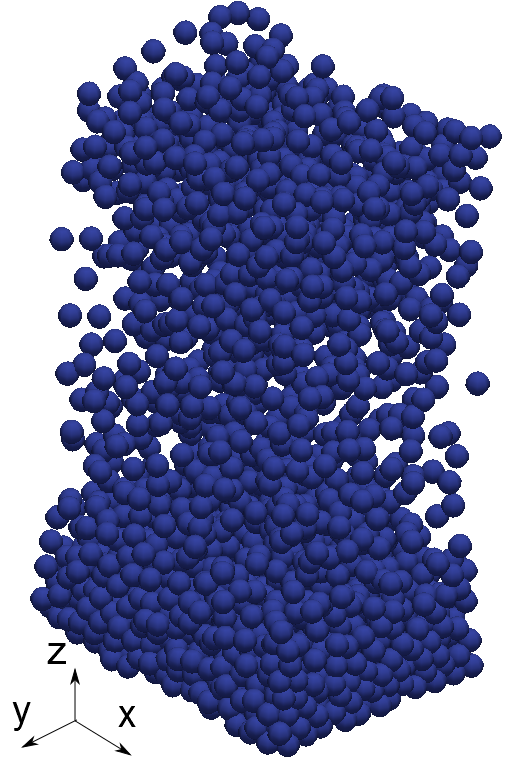
\includegraphics[width=\textwidth]{chapters/figures/fill01.png}
	\end{subfigure}
	\begin{subfigure}[b]{0.25\textwidth}
		\centering
		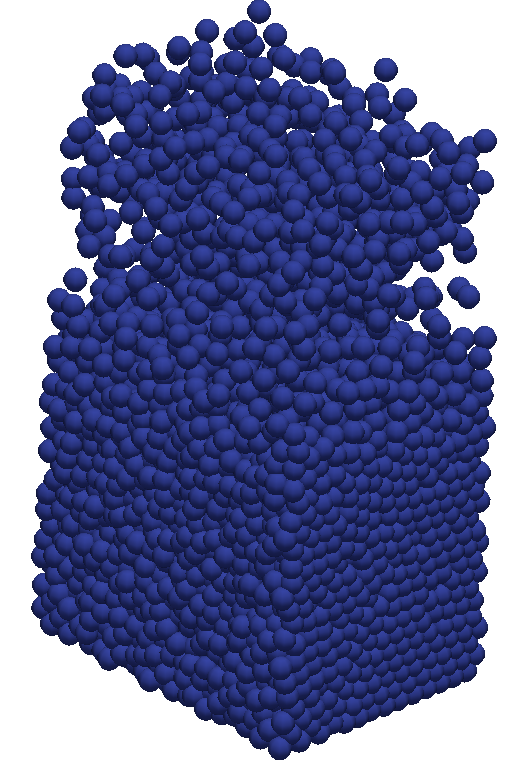
\includegraphics[width=\textwidth]{chapters/figures/fill02.png}
	\end{subfigure}
	\begin{subfigure}[b]{0.25\textwidth}
		\centering
		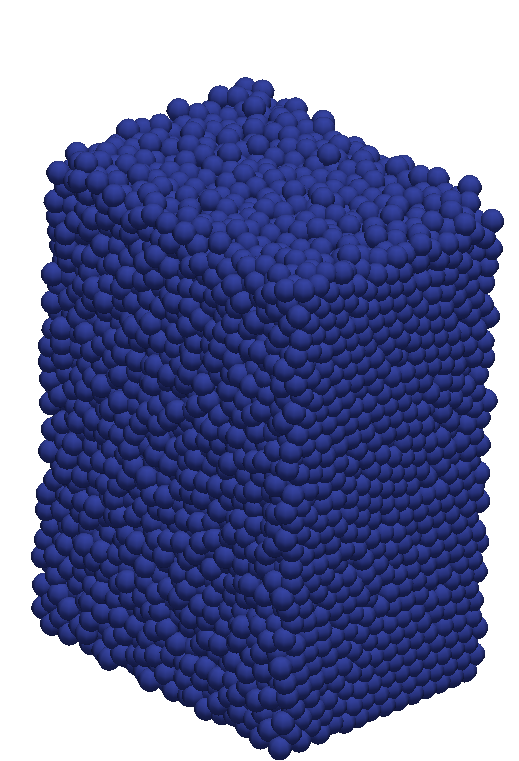
\includegraphics[width=\textwidth]{chapters/figures/fill03.png}
	\end{subfigure}
	\caption{Demonstrating the pouring process of $N = 10550$ pebbles into the control volume with at an early time (left), when it is nearly filled (middle) and after the pebbles have settled to negligible kinetic energy (right).}
\label{fig:fill01}
\end{figure}

In the end, a simpler pack-relax method was used instead. In this method $N$ particles are inserted into the volume such that we have precisely the packing fraction we desire (in this case, $\phi = 64\%$ so $N = 11000$). The pebbles are placed at random into the volume and are allowed to artificially overlap -- often by a great deal ($\delta \sim R_p$). The overlap they experience would normally cause such an enormous force (integrating into an enormous velocity) that the pebbles would all explode out of the bed at the first step in time integration. We avoid such a catostrophic scenario with a relaxation scheme where we truncate the displacement of any pebble per time step that is integrated from the force. The truncated displacement is very small and allows the pebbles to slowly move away from each other and into a static equilibirum as the artifical overlap is reduced. Once the pebble bed comes to rest, we remove the relaxation (limiting displacement command) and allow standard integration of contact forces with the velocity-Verlet algorithm (details in \cref{sec:dem-stability}). The pack-relax scheme allowed for obtaining desireable, highly repeatable packing fractions for all pebble beds. Once the pebble bed was packed into an initial condition, the simulation state was saved and used as a starting point for the numerous `crushed' cases to be described later.

In this first study, we model pebble crushing without considering why the particular pebble should be cracking. In the model we randomly select pebbles from the ensemble, regardless of forces acting upon the pebble, and delete them entirely from the system. When a pebble is removed, the neighboring pebbles react due to the imbalance of forces, and the bed settles into a new configuration. We differentiated the failed beds by their percentage of failed pebbles: $\eta = $ number of failed pebbles per original ensemble size. For the baseline case and for beds after failing, we apply the heating routine described next.

To simulate the conditions of a solid breeder in a fusion reactor, where the heat is removed from the pebble bed via contact to the containing structure, we assigned a constant temperature of $T_\text{c}$ to the vertical walls. Nuclear heating of the pebbles is simulated through a constant source term on each pebble. A representative heating rate of $Q_s = q_p'''V_p$, where  $q_p'''= 8$ MW/m$^3$. The heating cycle runs until a thermal steady state is reached. Based on a measurement of the total thermal energy of the bed, $E_T =\sum_i^N m_iC_i T_i$, steady-state is determined as $\dt{E_T} = 0$ within a specified tolerance. Once at steady state, we analyzed thermal and mechanical characteristics of the pebble bed: effective thermal conductivity, average coordination number, temperature profiles in the bed, and inter-particle contact forces. 

Based on the boundary conditions to our system, we establish heat transfer that is symmetric and one-dimensional in the $x$-direction from $x=0$ to the walls at $\frac{x}{d_p} = \pm 10$. As we will show, the pebble bed has very little variation of forces and temperatures in the $y$-direction due to the periodic boundary condition at the edges of the domain. Gravity effects are minor in the overall heat transfer and induce only a slight $z$-dependency to the results. We take advantage of this nature of our pebble bed to find the effective conductivity from an analytic, one-dimensional test case.
%~~~~~~~~~~~~~~~~~~~~~~~~~~~~~~~~~~~~~~~~~~~~~~~~~~~~~~~~~~~~~~~~~~~~~~





%~~~~~~~~~~~~~~~~~~~~~~~~~~~~~~~~~~~~~~~~~~~~~~~~~~~~~~~~~~~~~~~~~~~~~~
\subsection{Effective Thermal Conductivity from Analytic Analogy}
Assuming a one-dimensional pebble bed, to find an effective conductivity, we step back into a continuum mechanics formulation where the pebble bed can be represented as a slab of solid material. We can analytically solve for the temperature equation in a slab with heat generation, symmetry about the centerline, and a constant boundary temperature condition.

At steady-state, the temperature of a material with constant temperature boundary conditions ($T(L) = T_s$), constant thermal conductivity ($\keff$), and nuclear heating ($q'''$) obeys the following equation

\begin{equation}\label{eq:continuum-heateqn}
	0 = \frac{\mathrm{d}^2T}{\mathrm{d}x^2} + \frac{q'''}{\keff}
\end{equation}

We introduce a nondimensional temperature
\begin{equation}
	\theta = \frac{T(x) - T_s}{T_0 - T_s}
\end{equation}
where $T_0$ is the temperature at the centerline of this slab (a value we will find momentarily). The length is nondimensionalized as
\begin{equation}
	x^* = \frac{x}{L}
\end{equation}

Thus we can re-write Eq.~\ref{eq:continuum-heateqn} as
\begin{equation}\label{eq:continuum-heateqn-nondim}
	0 = \frac{\mathrm{d}^2\theta}{\mathrm{d}x^{*2}} + G
\end{equation}
where
\begin{equation}
	G = \frac{q'''L^2}{\keff(T_0 - T_s)}
\end{equation}

In the nondimensionalized form, the solution is revealed to be purely geometric,
\begin{equation}\label{eq:continuum-temperature-nondim}
	\theta = 1-x^{*2}
\end{equation}. 
as $T_0  - T_s = \frac{q'''L^2}{2\keff}$. We will use the nondimensional temperature solution of Eq.~\ref{eq:continuum-temperature-nondim} to prove our one-dimensional assumption of heat transfer is justified for the pebble beds.

We note that in this continuum mechanics formulation, we are assuming that the nuclear source, $q'''$ term is applied evenly over the entire volume. In our DEM formulation, our source term applies to a single pebble. To find the effective thermal conductivity of our `slab' of pebble bed, we must reconcile this discrepency. This is accomplished with the exchange of
\begin{equation}\label{eq:q-source-translation}
	q''' = \frac{Q_\text{tot}}{V_\text{tot}} = \frac{Q_sN}{H\cdot L\cdot W\cdot d_p^2}
\end{equation}
where the pebble bed volume is given by the height, $H$, width, $W$, and length, $L$, and $Q_s$ is the source term on each pebble in the DEM ensemble. 

From the solution of Eq.~\ref{eq:continuum-heateqn-nondim}, we find the effective conductivity to be
\begin{equation}
	\keff = \frac{q''' L^2}{2(T_0-T_s)}
\end{equation}
and when we replace the heat generation term with Eq.~\ref{eq:q-source-translation}, and use the bed dimensions as given in \cref{sec:dem-setup}, this is written as
\begin{equation}\label{eq:dem-effecitve-conductivity-formula}
	\keff = \frac{Q_sN}{180(T_0-T_s)d_p}
\end{equation}

We will use this formulation of Eq.~\ref{eq:dem-effecitve-conductivity-formula} to analyze and compare the pebble beds of this study.
% \begin{figure}[htbp]
% 	\centering
% 	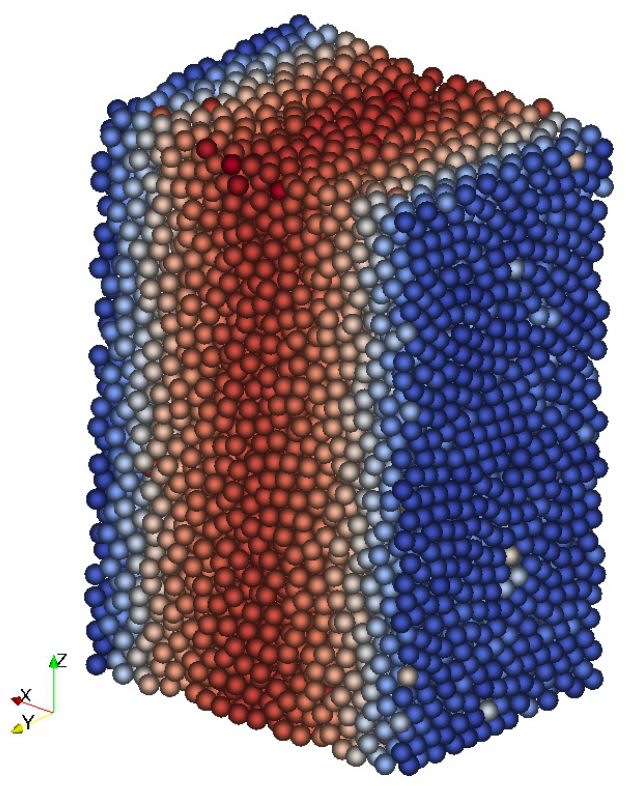
\includegraphics[trim=1cm 8cm 3cm 4cm, width=0.5\textwidth]{chapters/figures/pebbleBedTemperature}
% 	\caption{Temperature distribution of pebbles in the $10\%$ failed bed. At the end of steady-state heating, a one-dimensional profile is evident in all pebble beds studied here. The pebbles are receiving nuclear heating. Cooling proceeds through the pebbles in contact with the walls in the $x$-direction.}
% \label{fig:pebbleBedTemperature}
% \end{figure}



\subsection{Results}
The aim of this study was both to discover the impact of pebble failure on thermo-mechanical properties as well as determine the impact as a function of the number of failed pebbles. To satisfy the latter, we created beds with $\eta = 1\%$, $3\%$, $5\%$, $10\%$, and $15\%$ of pebbles failed. 

We plot Eq.~\ref{eq:continuum-temperature-nondim} against the nondimensionalized temperature profiles coming from the steady-state DEM simulation in Fig.~\ref{fig:temp-scatters}. We find that all our models had a nearly perfect match to a one-dimensional prediction, validating the calculation of effective thermal conductivity in this study. Furthmore, the profiles adhering to the one-dimensional curve also allows us to find the effective conductivity of each bed from applying Eq.~\ref{eq:dem-effecitve-conductivity-formula}, which was derived from the one-dimensional assumption.

In a well-packed bed, most pebbles have a coordination number $Z > 6$. But even in a well-packed bed, there exist some `rattlers' -- pebbles that have only 1 or 2 contact points (aside from touching the floor or wall). These rattlers, without strong contact to neighbors, heat up arbitrarily high in the system. In a pebble bed that's resettling due to damage, increased numbers of rattlers appear in the bed. The isolated rattlers are apparent in the scatter plots of Fig.~\ref{fig:temp-scatters}. The temperatures of most pebbles are tightly grouped around the parabolic average. Though many data points are seen dotted all around the temperature scale. The phenomena of hot rattlers is only possible when we use DEM without consideration of the helium purge gas. If these hot rattlers persist even in the presence of helium, it could lead to an unfavorable performance of the ceramic solid breeder -- the hot rattlers would sinter and prevent the outgassing of tritium among other issues. The observation of these isolated pebbles is another motivator for the coupling of DEM to thermo-fluid models. Because the 10\% and 15\% cases have such high temperatures, we show only the 0-5\% crushed together in Fig.~\ref{fig:temp-scatters-zoomed}

\begin{figure}[htbp]
	\centering
	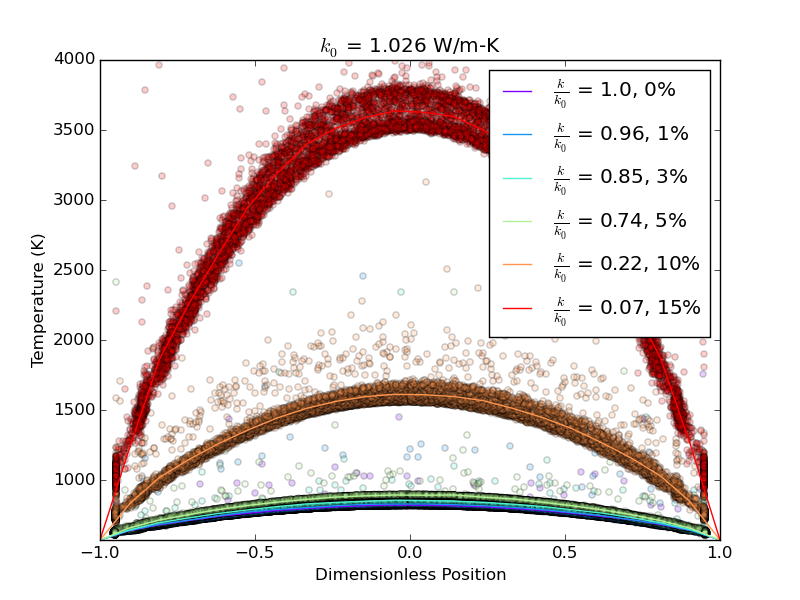
\includegraphics[width=\singleimagewidth]{chapters/figures/dem-evap-0-15-scatter-keff.png}
	\caption{The nondimensional temperature profiles for each test case follow the theoretical shape of a one-dimensional, constant $k$, continuum solution.}
\label{fig:temp-scatters}
\end{figure}

\begin{figure}[htbp]
	\centering
	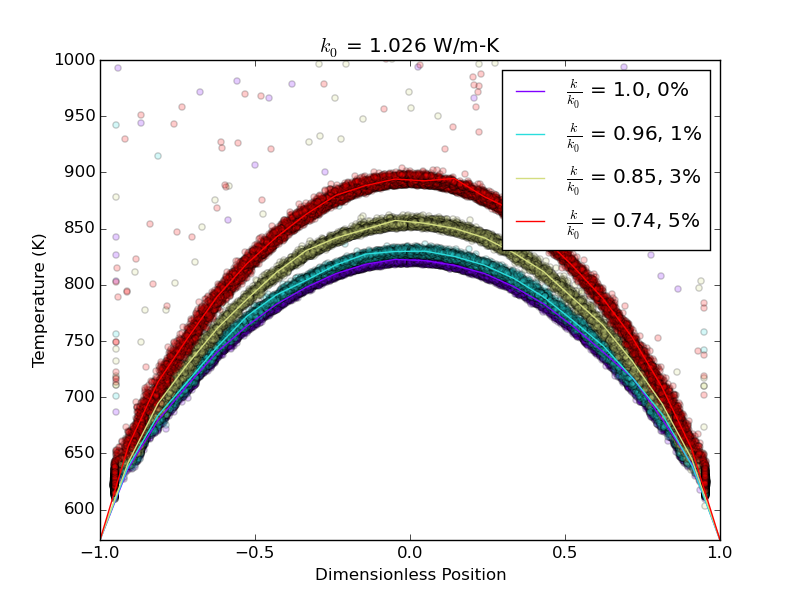
\includegraphics[width=\singleimagewidth]{chapters/figures/dem-evap-0-5-scatter-keff.png}
	\caption{The nondimensional temperature profiles for the test cases up to 5\% crushed pebbles.}
\label{fig:temp-scatters-zoomed}
\end{figure}


In order to calculate an effective conductivity of the pebble bed, we must find an average temperature profile through the bed to compare with Eq.~\ref{eq:continuum-temperature-nondim} and thus employ Eq.~\ref{eq:dem-effecitve-conductivity-formula}. We compare steady-state temperature profiles in the test beds against the one-dimensional, nondimensional temperature profile. Average values of the bed, along the $x$ direction, are generated via averaging temperatures in bins. We create bins that are volumes slices of width $\Delta x$ that extend through the limits of the $y$- and $z$-directions. We then find the $n$ pebbles residing in the slices and take the mean value of their temperatures. The average, given by Eq.~\ref{eq:binned-T}, is also given in Fig.~\ref{fig:temp-scatters}. The binned average temperature is 
\begin{equation}\label{eq:binned-T}
	\langle T\rangle = \frac{1}{n}\sum_{i}^n T_i 	
\end{equation}
Using the volume slices, we also find the average coordination number, 
\begin{equation}\label{eq:binned-z}
	\langle Z \rangle = \frac{1}{n}\sum_{i}^n Z_i
\end{equation}
and average contact force, 
\begin{equation}\label{eq:binned-f}
	\langle F^{1/3} \rangle = \frac{1}{n}\sum_{i}^n F_{n,ij}^{1/3}
\end{equation}


In Eq.~\ref{eq:thermoFirstLaw} of \cref{sec:dem-heat-transfer}, we see that at steady-state, the energy input by nuclear heating must be balanced by the transport of heat out of a pebble into its neighbors. Inter-particle heat transfer is dictated by the number of neighboring contacts, temperature difference between pebbles, and the thermal conductance, $H_{c}$, through the contact area. The thermal conductance (see Eq.~\ref{eq:dem-conductance}) is itself a function purely of material properties  (which are essentially constant here) and the force at the contact, going as $H_{c} \propto F_{n,ij}^{1/3}$. Thus, we write the net heat out of a pebble at steady state as a function of the three variables,

\begin{equation}
	Q_\text{net} =f( Z, F_n^{1/3}, \Delta T)
\end{equation}

The coordination number and contact forces are features of the packing structure in the packed bed that we can analyze to discover what happens to the heat flux between pebbles when the bed experiences crushed particles. Conversely, the $\Delta T$ between two pebbles is the effect of the thermal transport (i.e. leading to higher bed temperatures such as those of Fig.~\ref{fig:temp-scatters}). We will first analyze the changes to the coordination numbers of pebbles in the ensemble as pebbles crush.


\begin{figure}[!ht]
	\centering
	\begin{subfigure}[b]{\doubleimagewidth}
		\centering
		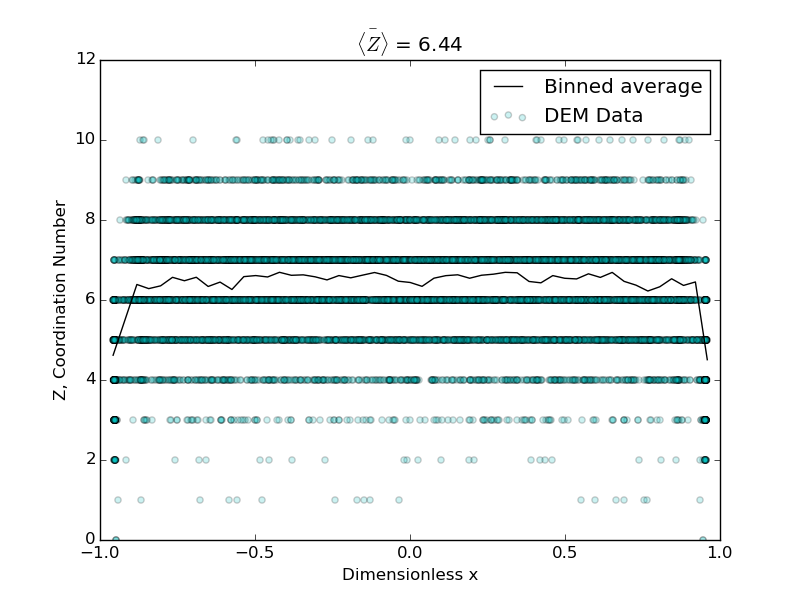
\includegraphics[width=\textwidth]{chapters/figures/heating_dte-02/dem-evap-0-scatter-coord.png}
		\caption{Baseline pebble bed (0\% crushed)}
	\end{subfigure}
	\begin{subfigure}[b]{\doubleimagewidth}
		\centering
		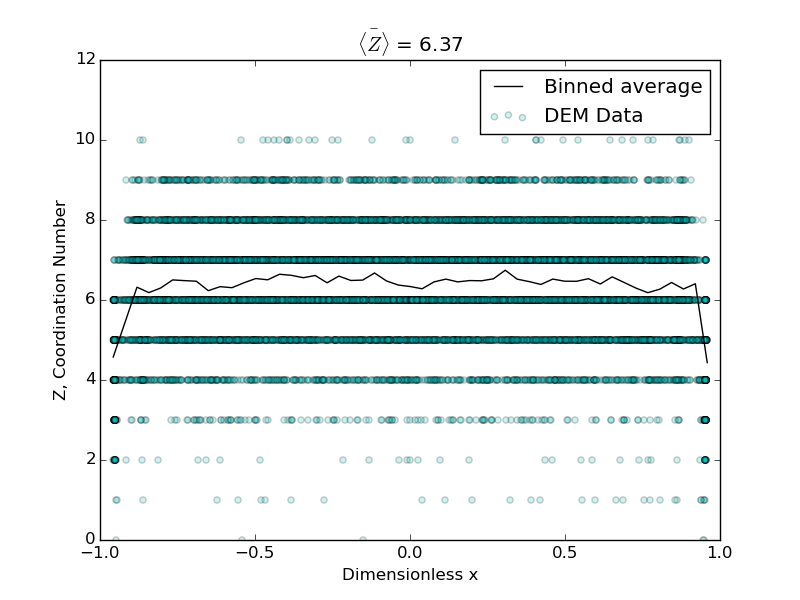
\includegraphics[width=\textwidth]{chapters/figures/heating_dte-02/dem-evap-1-scatter-coord.png}
		\caption{1\% crushed}
	\end{subfigure}
	
	\begin{subfigure}[b]{\doubleimagewidth}
		\centering
		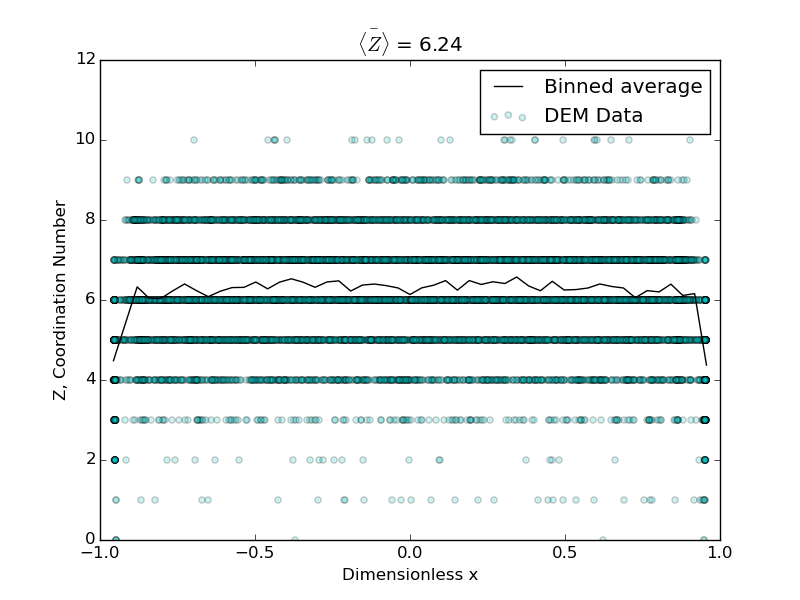
\includegraphics[width=\textwidth]{chapters/figures/heating_dte-02/dem-evap-2-scatter-coord.png}
		\caption{3\% crushed}
	\end{subfigure}
	\begin{subfigure}[b]{\doubleimagewidth}
		\centering
		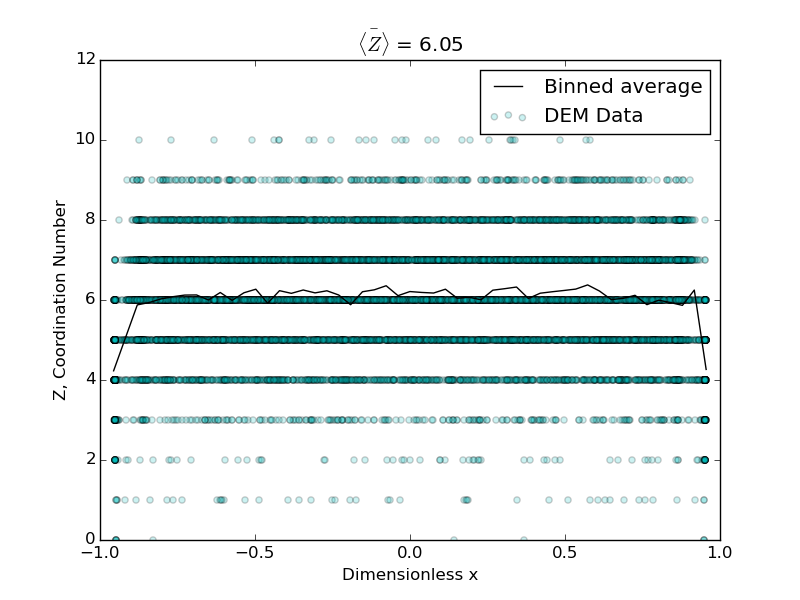
\includegraphics[width=\textwidth]{chapters/figures/heating_dte-02/dem-evap-3-scatter-coord.png}
		\caption{5\% crushed}
	\end{subfigure}

	\begin{subfigure}[b]{\doubleimagewidth}
		\centering
		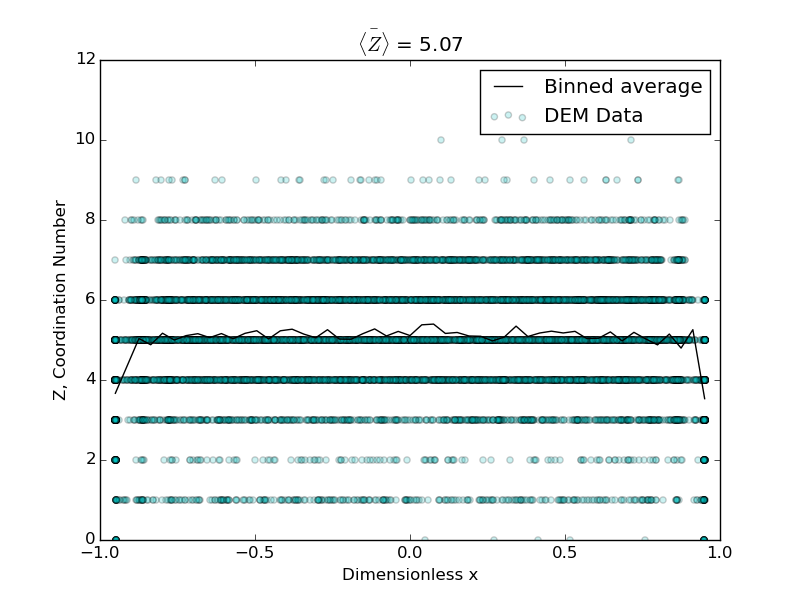
\includegraphics[width=\textwidth]{chapters/figures/heating_dte-02/dem-evap-4-scatter-coord.png}
		\caption{10\% crushed}
	\end{subfigure}
	\begin{subfigure}[b]{\doubleimagewidth}
		\centering
		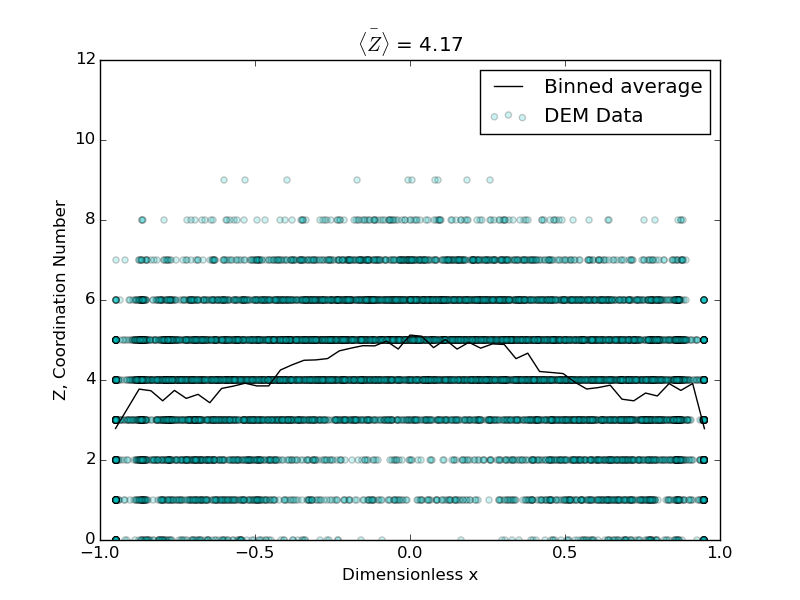
\includegraphics[width=\textwidth]{chapters/figures/heating_dte-02/dem-evap-5-scatter-coord.png}
		\caption{15\% crushed}\label{fig:coord-scatter-15percent}
	\end{subfigure}
	\caption{The average coordination number decreases slowly as the number of broken pebbles in the ensemble increases.}
\label{fig:coord-scatter}
\end{figure}

In Fig.~\ref{fig:coord-scatter} we plot the data for all pebbles in the ensemble as well as the binned average (Eq.~\ref{eq:binned-z}). Clearly, there are fewer average contacts per pebble in the ensemble after failure; At 15\% crushed the coordination number drops by roughly 30\%. But this alone can not not account for the reduction in $\keff$ by 93\% for the same amount of crushed pebbles. Next we look to the normal contact forces between pebbles in the bed.


\begin{figure}[!ht]
	\centering
	\begin{subfigure}[b]{0.4\textwidth}
		\centering
		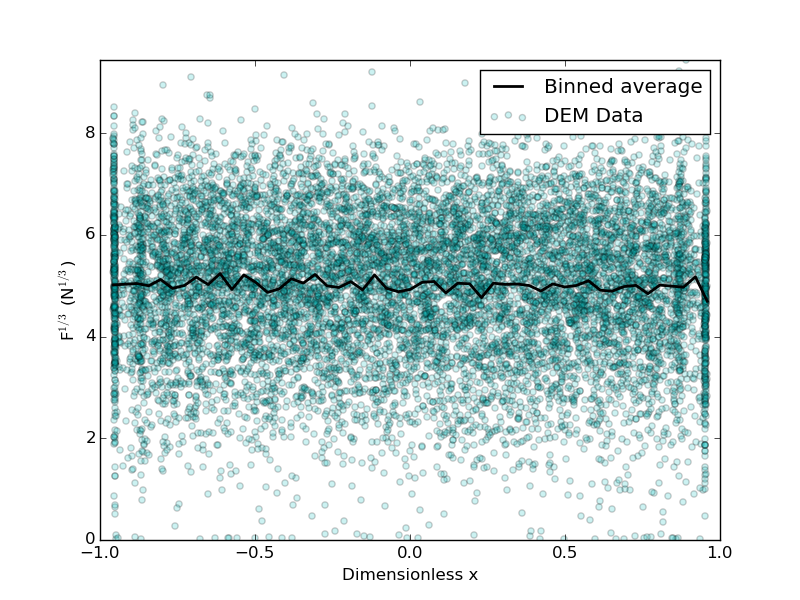
\includegraphics[width=\textwidth]{chapters/figures/heating_dte-02/0/dump/force-profile.png}
		\caption{Baseline pebble bed (0\% crushed)}
	\end{subfigure}
	\begin{subfigure}[b]{0.4\textwidth}
		\centering
		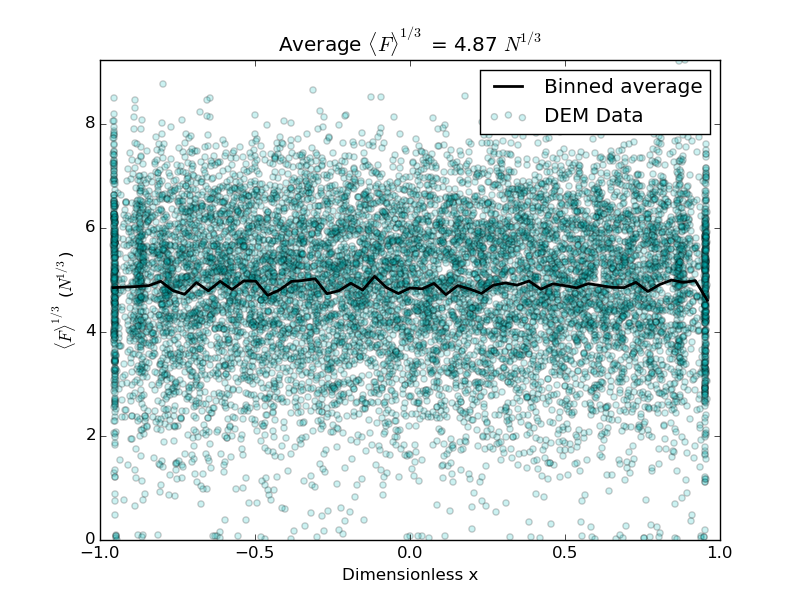
\includegraphics[width=\textwidth]{chapters/figures/heating_dte-02/1/dump/force-profile.png}
		\caption{1\% crushed}
	\end{subfigure}
	
	\begin{subfigure}[b]{0.4\textwidth}
		\centering
		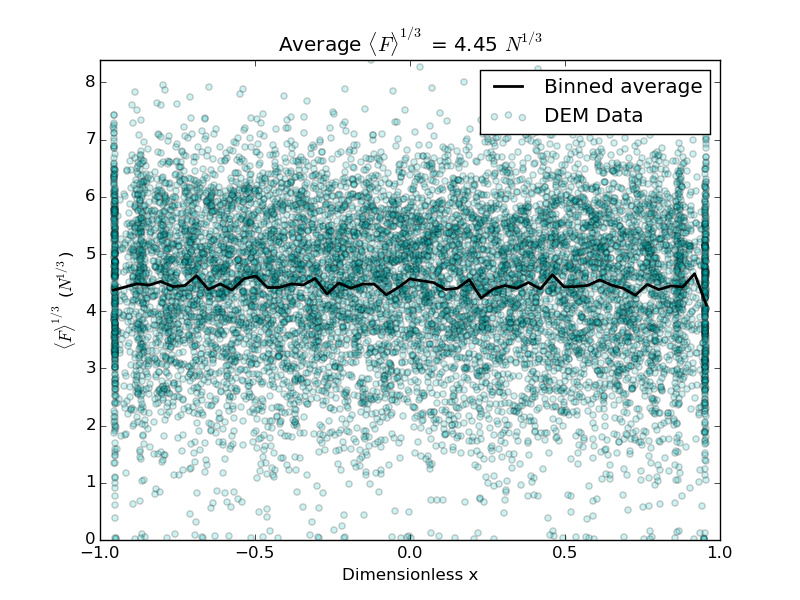
\includegraphics[width=\textwidth]{chapters/figures/heating_dte-02/3/dump/force-profile.png}
		\caption{3\% crushed}
	\end{subfigure}
	\begin{subfigure}[b]{0.4\textwidth}
		\centering
		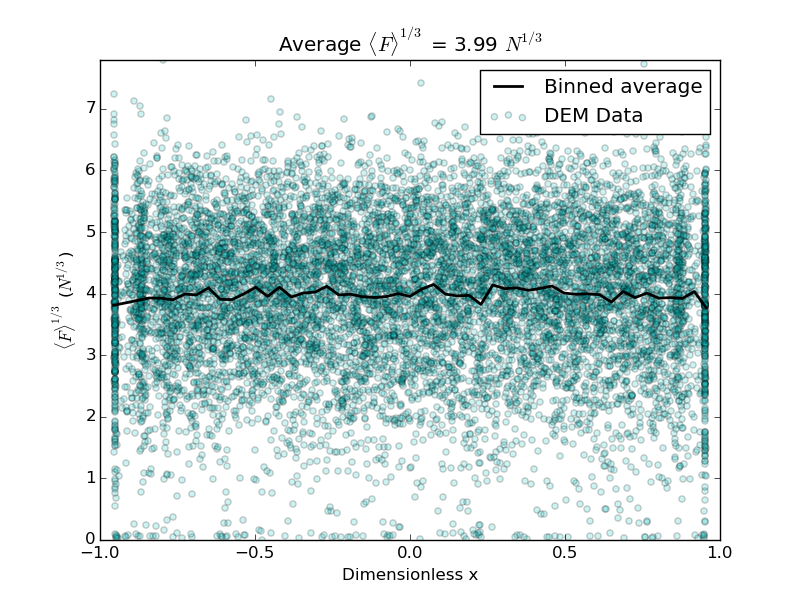
\includegraphics[width=\textwidth]{chapters/figures/heating_dte-02/5/dump/force-profile.png}
		\caption{5\% crushed}
	\end{subfigure}

	\begin{subfigure}[b]{0.4\textwidth}
		\centering
		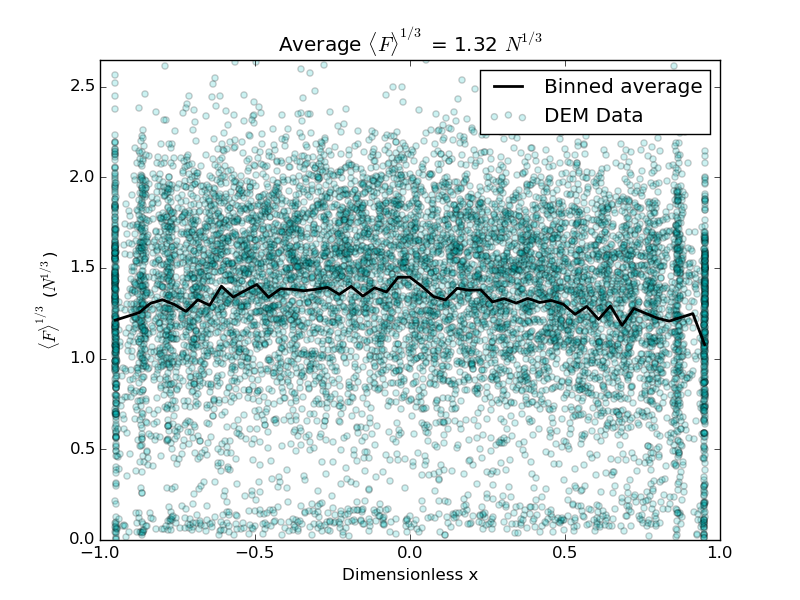
\includegraphics[width=\textwidth]{chapters/figures/heating_dte-02/10/dump/force-profile.png}
		\caption{10\% crushed}
	\end{subfigure}
	\begin{subfigure}[b]{0.4\textwidth}
		\centering
		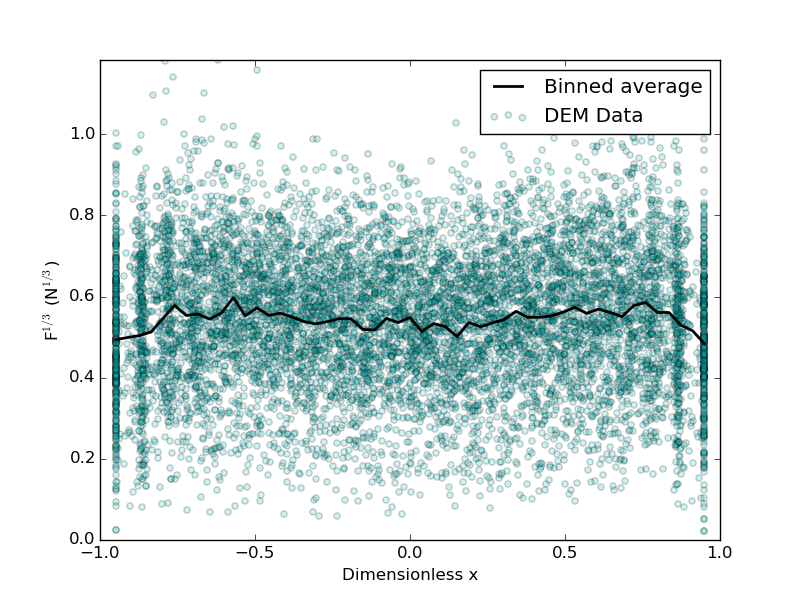
\includegraphics[width=\textwidth]{chapters/figures/heating_dte-02/15/dump/force-profile.png}
		\caption{15\% crushed}\label{fig:contact-forces-scatter-15percent}
	\end{subfigure}
	\caption{As pebble beds experience massive amounts of crushed pebbles (>5\%), the contact forces in the ensemble (after heating to steady-state) show dramatic reductions in value. Note the change of scale on the figures from the baseline case to the 15\% crushed case.}
\label{fig:contact-forces-scatter}
\end{figure}

The normal contact forces between pebbles are plotted in Fig.~\ref{fig:contact-forces-scatter}. A dramatic reduction in the normal forces is seen after many of their neighbors are crushed and are removed from the system. From the baseline down to the 15\% failed case, the contact forces are reduced by about a factor of 10 - similar to the reduction in effective conductivity.

The effective thermal conductivity was found for all of our pebble beds, via Eq.~\ref{eq:dem-effecitve-conductivity-formula}, then normalized against the conductivity of the baseline ensemble ($k^* = k/k_\text{0}$). The average coordination number of the beds and average normal contact forces were also found. Another way of describing a pebble bed is with the packing fraction, $\phi$. In Fig.~\ref{fig:packing-fraction}, we collect all these values (and normalize them against the baseline case) to provide a direct comparison to their changes as a function of crushed pebbles. When $15\%$ of the pebbles are crushed in a pebble bed, the effective conductivity has fallen all the way to only $k^*=0.07$. This large reduction is especially important in light of the already poor thermal management of virgin pebble beds that, even in helium environments, have been experimentally measured at only approximately 1~W/m-K (see, \textit{ e.g.}, Refs.~\cite{Reimann:2002mi, Piazza2002811}). The only parameter to have similar reductions in value is the average normal contact force, a value which is seen to follow closely to the curve of effective conductivity. Thus we conclude that the single most important factor for determining the effective thermal conductivity in these pebble beds is the normal contact forces between pebbles; a force which decreases sharply as pebbles are crushed in the system.

\begin{figure}[!ht]
	\centering
	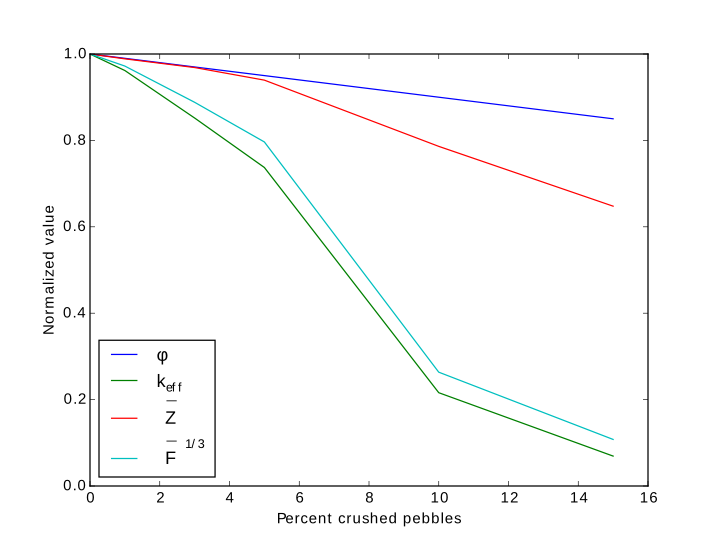
\includegraphics[width=\singleimagewidth]{chapters/figures/kEff_packingFraction}
	\caption{The normalized effective conductivity drops much more rapidly than the normalized packing fraction, $\phi$, while pebbles are crushed. The effective conductivity follows with reduced normal contact forces.}
\label{fig:packing-fraction}
\end{figure}

The large reduction in normal contact force (which leads to a large reduction in effective conductivity) is explainable based on the experimental setup of our numeric model. In our system, we had rigid walls in the $x$ and $z$ directions. These walls did not change after the substantial number of pebbles were crushed and removed. After the 15\% crushing event, the pebble bed appeared as Fig.~\ref{fig:15percent-crushed-pre}. A massive re-arrangement proceeds from the crushing event. As the pebble bed heats up, the thermal expansion of the pebbles is unconstrained as there exists an average of two pebble diameter gap above the pebbles to the top of the container. Numerically there is no limit to the pebble temperatures (phase change and sintering is not incorporated into the DEM calculations) so the pebbles heat and swell until coming into contact with the top wall, at which time they begin to press into one another (though lightly) to allow thermal conduction. The pebble bed after swelling is shown in Fig.~\ref{fig:15percent-crushed-swelling}.

\begin{figure}[!ht]
	\centering
	\begin{subfigure}[t]{\doubleimagewidth}
		\centering
		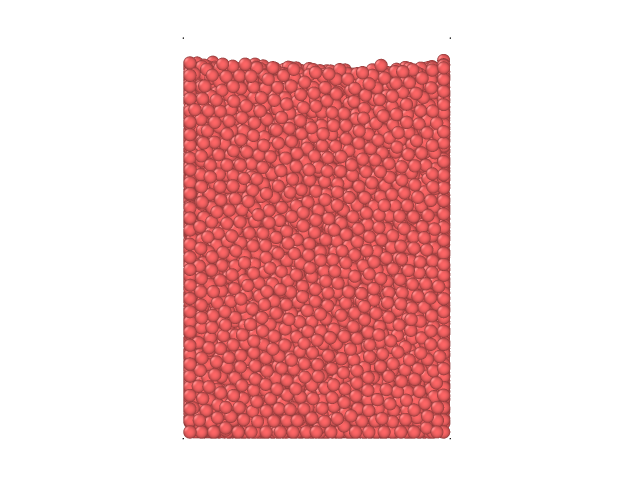
\includegraphics[width=\textwidth]{chapters/figures/heating_dte-02/15/0.15_pre_heat.png}
		\caption{Side-view of the pebble bed after resettling from the crushing event, before heating.}
		\label{fig:15percent-crushed-pre}
	\end{subfigure}
	\begin{subfigure}[t]{\doubleimagewidth}
		\centering
		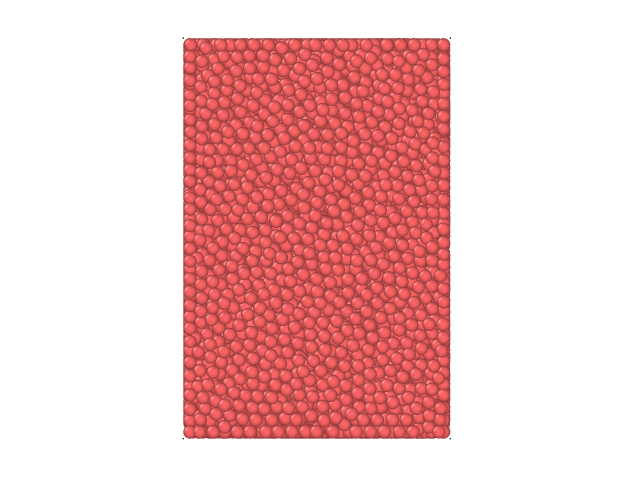
\includegraphics[width=\textwidth]{chapters/figures/heating_dte-02/15/0.15_post_heat.png}
		\caption{Side-view of the pebble bed after heating}
		\label{fig:15percent-crushed-swelling}
	\end{subfigure}
	\caption{In (a) we see the pebble bed after 15\% of the pebbles have been crushed (removed) and then after the heating cycle in (b). The gap formed after crushing is completely filled by swelling pebbles.}
\end{figure}

One last note that must be made concerning this study is on the initial packing state. As the first study performed with our new numeric tools, we were unaware of some of the measures of describing a pebble bed. For instance, we desired to match the experimental setup of our laboratory insomuch as matching general dimensions and packing fractions. What we did not realize, however, was that forcing our pebble bed to achieve a pre-determined packing fraction at the expense of ignoring initial inter-particle contact forces was improper. The error of this initial packing is immediately seen when we compare the $\keff$ of our baseline pebble bed with those of experiments, shown back in Fig.~\ref{fig:keff-pressure}. Our pebble bed, in the absence of helium, ought to have had an effective thermal conductivity close to $\keff = 0.2$~W/m-K. What we found, however was an initial $\keff = 1.026$~W/m-K.

Returning to this study, I attempted to assemble new pebble beds with different initial packing techniques. Instead of imitating the vibration-roof-pressing technique from the laboratory, I created an artificial packing technique. In this technique, the particles are all initially without contact friction and gravity was not turned on in the system. The limits of the periodic dimension were increased dramatically and the pebbles were allowed to fill the void space with large spaces in between. Then, slowly, the periodic boundaries shrunk which compressed the pebble bed. The frictionless, weightless pebbles were free to move around each other to create large packing fractions (up to $\phi = 64\%$) with minimal initial contact forces. These newly-packed pebble beds were again run to a thermal steady-state and an effective conductivity value established. In these cases, the initial $\keff$ was much closer to the values expected from physical experiments. The results of the contact forces in a number of new beds are given in Fig.~\ref{fig:contact-forces-scatter-initial}. The smaller initial contact forces lead to effective conductivities as shown in Fig.~\ref{fig:keff-initial}. If these new initial values of $\keff$ are compared to the damaged cases, the percent decrease in $\keff$ reported would be doubled. The results of these new packing techniques highlight the importance of the initial packing of the pebble bed when it comes to interpreting the output of the data. That is to say, neither of the results given are more correct or more incorrect than the other. They are simply more or less applicable to situations that have the same initial conditions -- including initial packing fraction and initial contact force.

\begin{figure}[!ht]
	\centering
	\begin{subfigure}[b]{0.4\textwidth}
		\centering
		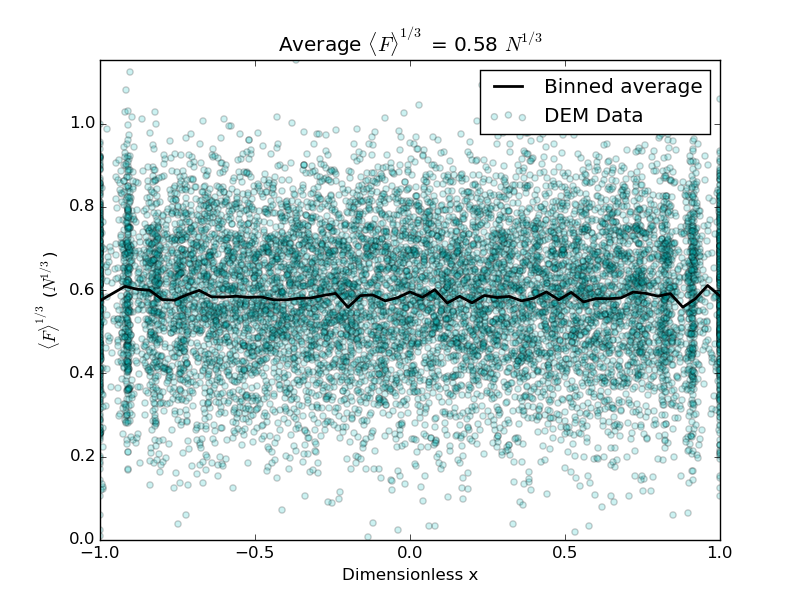
\includegraphics[width=\textwidth]{chapters/figures/initial_packing_study/62-deform-force-profile.png}
		\caption{Packed to $\phi = 62$\%}
	\end{subfigure}
	
	\begin{subfigure}[b]{0.4\textwidth}
		\centering
		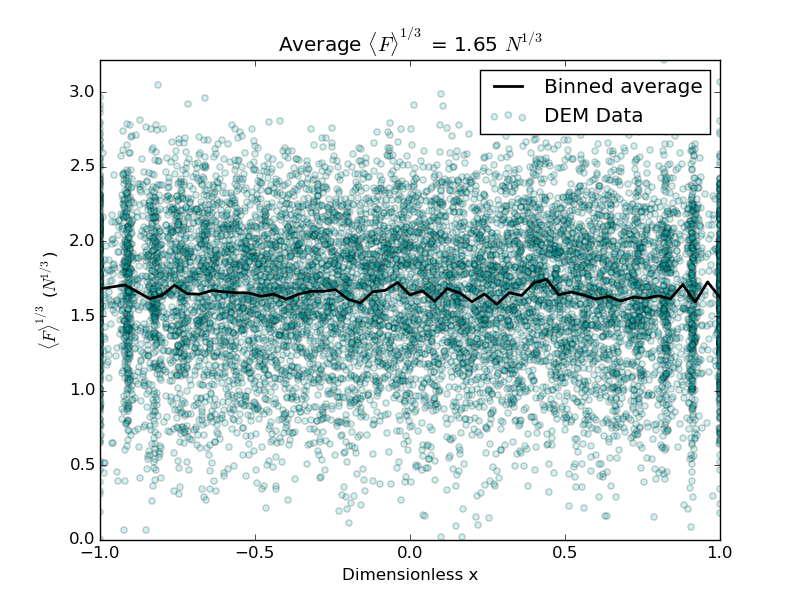
\includegraphics[width=\textwidth]{chapters/figures/initial_packing_study/63-deform-force-profile.png}
		\caption{Packed to $\phi = 63$\%}
	\end{subfigure}

	\begin{subfigure}[b]{0.4\textwidth}
		\centering
		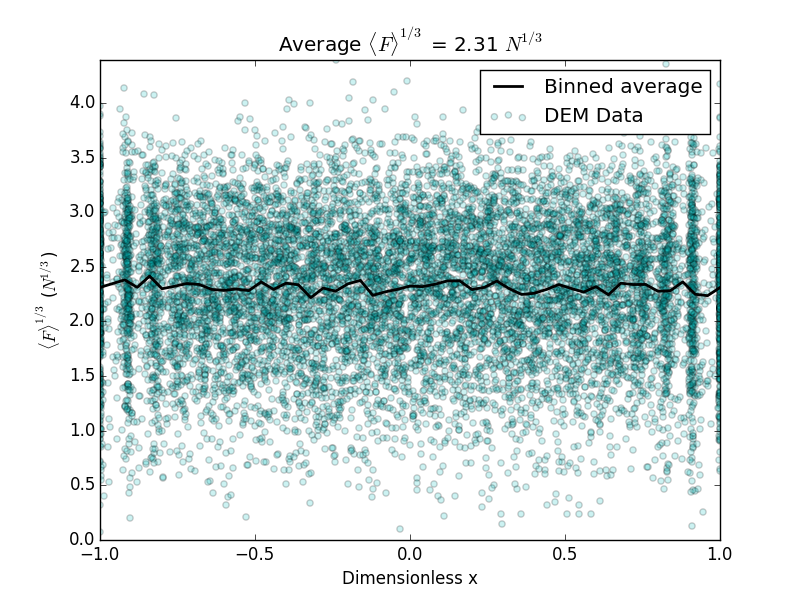
\includegraphics[width=\textwidth]{chapters/figures/initial_packing_study/64-deform-force-profile.png}
		\caption{Packed to $\phi = 64$\%}
	\end{subfigure}
	\caption{Initial force distributions in pebble beds packed with a new routine.}
\label{fig:contact-forces-scatter-initial}
\end{figure}

\begin{figure}[!ht]
	\centering
	\begin{subfigure}[b]{0.4\textwidth}
		\centering
		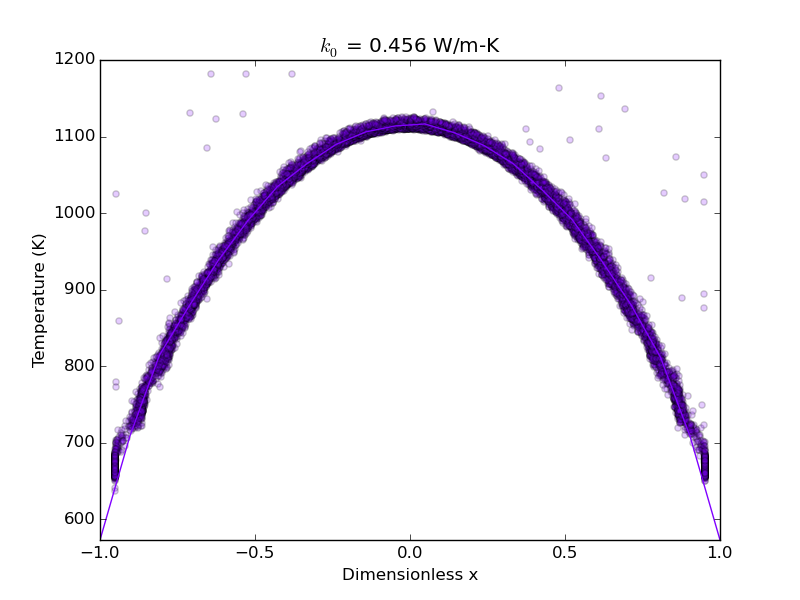
\includegraphics[width=\textwidth]{chapters/figures/initial_packing_study/62percent-deform-packing.png}
		\caption{Packed to $\phi = 62\%$}
	\end{subfigure}
	
	\begin{subfigure}[b]{0.4\textwidth}
		\centering
		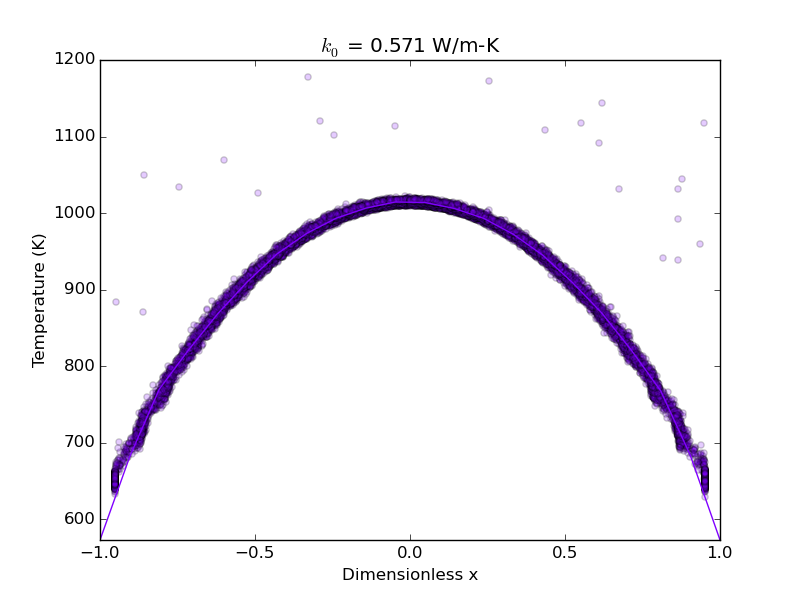
\includegraphics[width=\textwidth]{chapters/figures/initial_packing_study/63percent-deform-packing.png}
		\caption{Packed to $\phi = 63\%$}
	\end{subfigure}

	\begin{subfigure}[b]{0.4\textwidth}
		\centering
		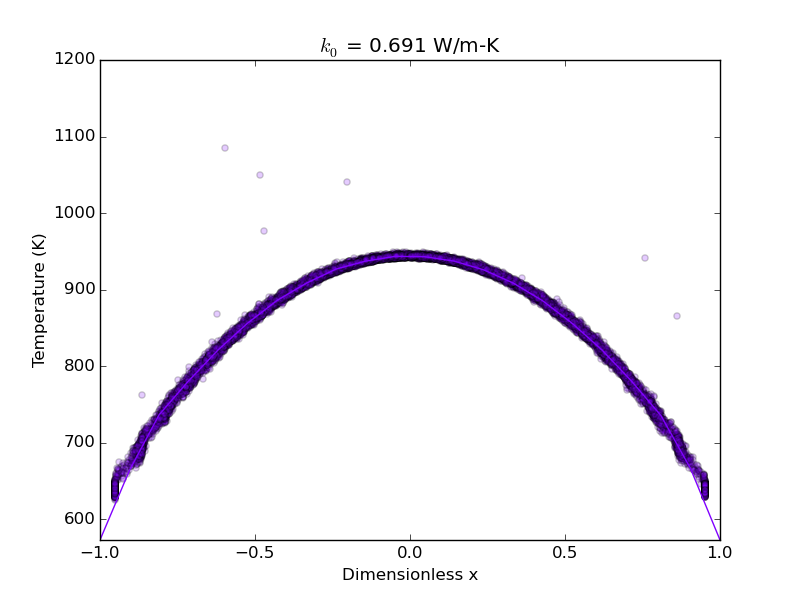
\includegraphics[width=\textwidth]{chapters/figures/initial_packing_study/64percent-deform-packing.png}
		\caption{Packed to $\phi = 64\%$}
	\end{subfigure}
	\caption{Initial $\keff$ in the lightly-packed pebble beds are much closer to values measured in experiments in vacuum.}
\label{fig:keff-initial}
\end{figure}





\FloatBarrier